
\documentclass[12pt, a4paper]{report}
\usepackage{natbib}
\usepackage{vmargin}
\usepackage{graphicx}
\usepackage{epsfig}
\usepackage{subfigure}
%\usepackage{amscd}
\usepackage{amssymb}
\usepackage{subfigure}
\usepackage{amsbsy}
\usepackage{amsthm, amsmath}
%\usepackage[dvips]{graphicx}
\bibliographystyle{chicago}
\renewcommand{\baselinestretch}{1.8}

% left top textwidth textheight headheight % headsep footheight footskip
\setmargins{3.0cm}{2.5cm}{15.5 cm}{23.5cm}{0.5cm}{0cm}{1cm}{1cm}

\pagenumbering{arabic}


\begin{document}
\author{Kevin O'Brien}
\title{Transfer Report}
\date{\today}
\maketitle

\tableofcontents \setcounter{tocdepth}{2}

\newpage
\chapter{Introduction}

\section{Introduction}
The problem of assessing the agreement between two or more methods
of measurement is ubiquitous in scientific research, and is
commonly referred to as a `method comparison study'. Published
examples of method comparison studies can be found in disciplines
as diverse as Pharmacology \citep{ludbrook97}, Anaesthesia
\citep{Myles}, and cardiac imaging methods \citep{Krumm}.
\smallskip

To illustrate the characteristics of a typical method comparison
study consider the data in Table I \citep{Grubbs73}. In each of
twelve experimental trials a single round of ammunition was fired
from a 155mm gun, and its velocity was measured simultaneously
(and independently) by three chronographs devices, identified here
by the labels `Fotobalk', `Counter' and `Terma'.
\smallskip


\newpage

\begin{table}[ht]
\begin{center}
\begin{tabular}{rrrr}
  \hline
  Round& Fotobalk [F] & Counter [C]& Terma [T]\\
  \hline
  1 & 793.8 & 794.6 & 793.2 \\
  2 & 793.1 & 793.9 & 793.3 \\
  3 & 792.4 & 793.2 & 792.6 \\
  4 & 794.0 & 794.0 & 793.8 \\
  5 & 791.4 & 792.2 & 791.6 \\
  6 & 792.4 & 793.1 & 791.6 \\
  7 & 791.7 & 792.4 & 791.6 \\
  8 & 792.3 & 792.8 & 792.4 \\
  9 & 789.6 & 790.2 & 788.5 \\
  10 & 794.4 & 795.0 & 794.7 \\
  11 & 790.9 & 791.6 & 791.3 \\
  12 & 793.5 & 793.8 & 793.5 \\
   \hline
\end{tabular}
\caption{Velocity measurement from the three chronographs (Grubbs
1973).}
\end{center}
\end{table}

An important aspect of the these data is that all three methods of
measurement are assumed to have an attended measurement error, and
the velocities reported in Table 1.1 can not be assumed to be
`true values' in any absolute sense.

%While lack of
%agreement between two methods is inevitable, the question , as
%posed by \citet{BA83}, is 'do the two methods of measurement agree
%sufficiently closely?'

A method of measurement should ideally be both accurate and
precise. \citet{Barnhart} describes agreement as being a broader
term that contains both of those qualities. An accurate
measurement method will give results close to the unknown `true
value'. The precision of a method is indicated by how tightly
measurements obtained under identical conditions are distributed
around their mean measurement value. A precise and accurate method
will yield results consistently close to the true value. Of course
a method may be accurate, but not precise. If the average of its
measurements is close to the true value, but those measurements
are highly dispersed. Conversely a method that is not accurate may
be quite precise, as it consistently indicates the same level of
inaccuracy. The tendency of a method of measurement to
consistently give results above or below the true value is a
source of systematic bias. The smaller the systematic bias, the
greater the accuracy of the method.


The FDA define precision as the closeness of agreement (degree of
scatter) between a series of measurements obtained from multiple
sampling of the same homogeneous sample under prescribed
conditions. \citet{Barnhart} describes precision as being further
subdivided as either within-run, intra-batch precision or
repeatability (which assesses precision during a single analytical
run), or between-run, inter-batch precision or repeatability
(which measures precision over time)

In the context of the agreement of two methods, there is also a
tendency of one measurement method to consistently give results
above or below the other method. Lack of agreement is a
consequence of the existence of `inter-method bias'. For two
methods to be considered in good agreement, the inter-method bias
should be in the region of zero. A simple estimation of the
inter-method bias can be calculated using the differences of the
paired measurements. The data in Table 1.2 are a good example of
possible inter-method bias; the `Fotobalk' consistently recording
smaller velocities than the `Counter' method. Consequently one
would conclude that there is lack of agreement between the two
methods.

The absence of inter-method bias by itself is not sufficient to
establish whether two measurement methods agree. The two
methods must also have equivalent levels of precision. Should one
method yield results considerably more variable than that of the
other, they can not be considered to be in agreement. With this in
mind a methodology is required that allows an analyst to estimate
the inter-method bias, and to compare the precision of both
methods of measurement.
\newpage
% latex table generated in R 2.6.0 by xtable 1.5-5 package
% Wed Aug 26 15:22:41 2009
\begin{table}[h!]

\begin{center}

\begin{tabular}{rrrr}
  \hline
 Round& Fotobalk (F) & Counter (C) & F-C \\
  \hline
1 & 793.8& 794.6 & -0.8 \\
  2 & 793.1 & 793.9 & -0.8 \\
  3 & 792.4 & 793.2 & -0.8 \\
  4 & 794.0 & 794.0 & 0.0 \\
  5 & 791.4 & 792.2 & -0.8 \\
  6 & 792.4 & 793.1 & -0.7 \\
  7 & 791.7 & 792.4 & -0.7 \\
  8 & 792.3 & 792.8 & -0.5 \\
  9 & 789.6 & 790.2 & -0.6 \\
  10 & 794.4 & 795.0 & -0.6 \\
  11 & 790.9 & 791.6 & -0.7 \\
  12 & 793.5 & 793.8 & -0.3 \\
   \hline
\end{tabular}
\caption{Difference between Fotobalk and Counter measurements.}
\end{center}
\end{table}

\bigskip


%%%%%%%%%%%%%%%%%%%%%%%%%%%%%%%%%%%%%%%%%%%%%%%%%%%%%%%%%%%%%%%%%%%%%%%%%%%%%%%%%%%%%%
%\newpage
\section{Bland-Altman Plots}
The issue of whether two measurement methods comparable to the
extent that they can be used interchangeably with sufficient
accuracy is encountered frequently in scientific research.
Historically comparison of two methods of measurement was carried
out by use of paired sample t-test, correlation coefficients or
simple linear regression. Statisticians Martin Bland and Douglas
Altman recognized the inadequacies of these analyses and
articulated quite thoroughly the basis on which of which they are
unsuitable for comparing two methods of measurement \citep*{BA83}.
Furthermore they proposed their simple methodology specifically
constructed for method comparison studies. They acknowledge the
opportunity to apply other valid, but complex, methodologies, but
argue that a simple approach is preferable, especially when the
results must be `explained to non-statisticians'.

Notwithstanding previous remarks about regression, the first step
recommended, which the authors argue should be mandatory, is
construction of a simple scatter plot of the data. The line of
equality should also be shown, as it is necessary to give the
correct interpretation of how both methods compare. A scatter plot
of the Grubbs data is shown in Figure 1.1. Visual inspection confirms the previous conclusion that there is an
inter-method bias present, i.e. Fotobalk device has a tendency to
record a lower velocity.

\begin{figure}[h!]
\begin{center}
  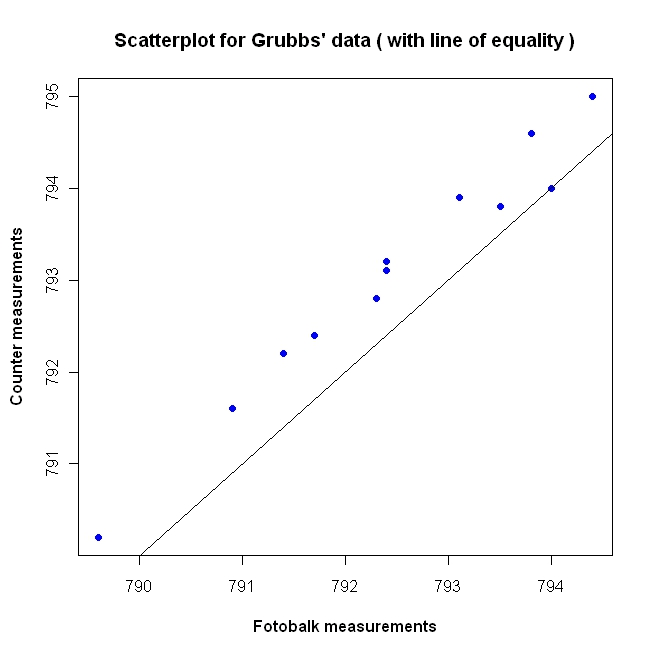
\includegraphics[width=130mm]{GrubbsScatter.jpeg}
  \caption{Scatter plot For Fotobalk and Counter Methods.}\label{GrubbsScatter}
\end{center}
\end{figure}

In light of shortcomings associated with scatterplots,
\citet*{BA83} recommend a further analysis of the data. Firstly
case-wise differences of measurements of two methods $d_{i} =
y_{1i}-y_{2i} \mbox{ for }i=1,2,..n$ on the same subject should be
calculated, and then the average of those measurements ($a_{i} =
(y_{1i} + y_{2i})/2 \mbox{ for }i=1,2,..n$). These differences and
averages are then plotted. This methodology, now commonly known as
the `Bland-Altman Plot', has proved very successful.
\citet*{BA86}, which further develops the methodology, was found
to be the sixth most cited paper of all time by the
\citet{BAcite}. \cite{Dewitte} also commented on the rate at which
prevalence of the Bland-Altman plot has developed in scientific
literature. The Bland-Altman Plot has since become expected, and
often obligatory, approach for presenting method comparison
studies in many scientific journals \citep{hollis}. Furthermore
\citet{BritHypSoc} recommend its use in papers pertaining to
method comparison studies for the journal of the British
Hypertension Society.

The magnitude of the inter-method bias between the two methods is
simply the average of the differences $\bar{d}$. The variances
around this bias is estimated by the standard deviation of the
differences $S(d)$. This inter-method bias is represented with a
line on the Bland-Altman plot. These estimates are only meaningful
if there is uniform inter-bias and variability throughout the
range of measurements, which can be checked by visual inspection
of the plot. In the case of Grubbs data the inter-method bias is
$-0.61$ metres per second, and is indicated by the dashed line on
Figure 1.2. By inspection of the plot, it is also possible to
compare the precision of each method. Noticeably the differences
tend to increase as the averages increase.


\begin{table}[h!]
\renewcommand\arraystretch{0.7}%
\begin{center}
\begin{tabular}{|c||c|c||c|c|}
  \hline
 Round & Fotobalk  & Counter  & Differences  & Averages  \\
  &  [F] & [C] & [F-C] &  [(F+C)/2] \\
  \hline
1 & 793.8 & 794.6 & -0.8 & 794.2 \\
  2 & 793.1 & 793.9 & -0.8 & 793.5 \\
  3 & 792.4 & 793.2 & -0.8 & 792.8 \\
  4 & 794.0 & 794.0 & 0.0 & 794.0 \\
  5 & 791.4 & 792.2 & -0.8 & 791.8 \\
  6 & 792.4 & 793.1 & -0.7 & 792.8 \\
  7 & 791.7 & 792.4 & -0.7 & 792.0 \\
  8 & 792.3 & 792.8 & -0.5 & 792.5 \\
  9 & 789.6 & 790.2 & -0.6 & 789.9 \\
  10 & 794.4 & 795.0 & -0.6 & 794.7 \\
  11 & 790.9 & 791.6 & -0.7 & 791.2 \\
  12 & 793.5 & 793.8 & -0.3 & 793.6 \\
   \hline
\end{tabular}
\caption{Fotobalk and Counter methods: differences and averages.}
\end{center}
\end{table}

\begin{table}[h!]
\renewcommand\arraystretch{0.7}%
\begin{center}
\begin{tabular}{|c||c|c||c|c|}
  \hline
 Round & Fotobalk  & Terma  & Differences  & Averages  \\
  &  [F] & [T] & [F-T] &  [(F+T)/2] \\
  \hline
1 & 793.80 & 793.20 & 0.60 & 793.50 \\
  2 & 793.10 & 793.30 & -0.20 & 793.20 \\
  3 & 792.40 & 792.60 & -0.20 & 792.50 \\
  4 & 794.00 & 793.80 & 0.20 & 793.90 \\
  5 & 791.40 & 791.60 & -0.20 & 791.50 \\
  6 & 792.40 & 791.60 & 0.80 & 792.00 \\
  7 & 791.70 & 791.60 & 0.10 & 791.65 \\
  8 & 792.30 & 792.40 & -0.10 & 792.35 \\
  9 & 789.60 & 788.50 & 1.10 & 789.05 \\
  10 & 794.40 & 794.70 & -0.30 & 794.55 \\
  11 & 790.90 & 791.30 & -0.40 & 791.10 \\
  12 & 793.50 & 793.50 & 0.00 & 793.50 \\

   \hline
\end{tabular}
\caption{Fotobalk and Terma methods: differences and averages.}
\end{center}
\end{table}

\newpage


\subsection{Using Bland-Altman Plots}
Bland-Altman plots are a powerful graphical methodology for making
a visual assessment of the data. \citet*{BA83} express the
motivation for this plot thusly:
\begin{quote}
``From this type of plot it is much easier to assess the magnitude
of disagreement (both error and bias), spot outliers, and see
whether there is any trend, for example an increase in
(difference) for high values. This way of plotting the data is a
very powerful way of displaying the results of a method comparison
study."
\end{quote}

The Bland-Altman plot is simply a scatterplot of the case-wise
averages and differences of two methods of measurement. As the
objective of the Bland-Altman plot is to advise on the agreement
of two methods, it is the case-wise differences that are
particularly. Later it will be shown that case-wise differences
are the sole component of the next part of the methodology, the
limits of agreement.

For creating plots, the case wise-averages fulfil several
functions, such as expressing the range over which the values were
taken, and assessing whether the assumptions of constant variance
holds. Case-wise averages also allow the case-wise differences to
be presented on a two-dimensional plot, with better data
visualization qualities than a one dimensional plot. \citet{BA86}
cautions that it would be the difference against either
measurement value instead of their average , as the difference
relates to both value.

The Bland-Altman plot for comparing the `Fotobalk' and `Counter'
methods, which shall henceforth be referred to as the `F vs C'
comparison,  is depicted in Figure 1.2, using data from Table 1.3.
The presence and magnitude of the inter-method bias is indicated
by the dashed line.

\begin{figure}[h!]
\begin{center}
  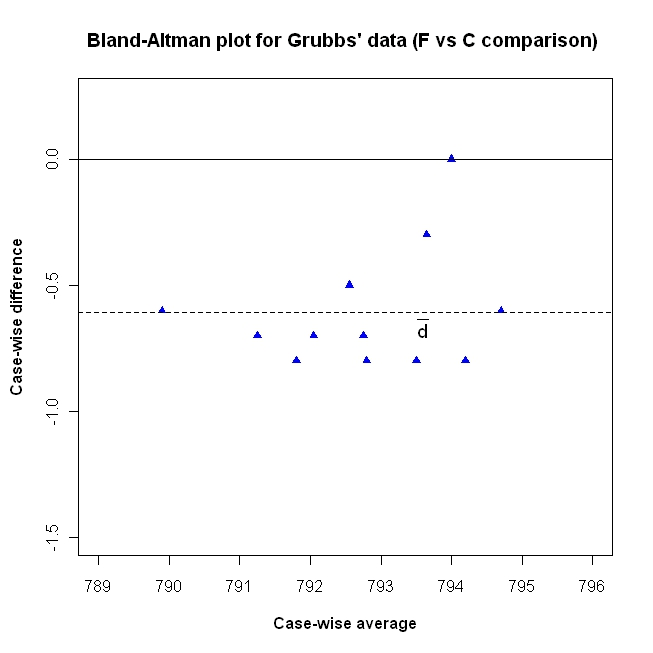
\includegraphics[width=120mm]{GrubbsBAplot-noLOA.jpeg}
  \caption{Bland-Altman plot For Fotobalk and Counter methods.}\label{GrubbsBA-noLOA}
\end{center}
\end{figure}



In Figure 1.3 Bland-Altman plots for the `F vs C' and `F vs T'
comparisons are shown, where `F vs T' refers to the comparison of
the `Fotobalk' and `Terma' methods. Usage of the Bland-Altman plot
can be demonstrate in the contrast between these comparisons.

\begin{figure}[h!]
\begin{center}
  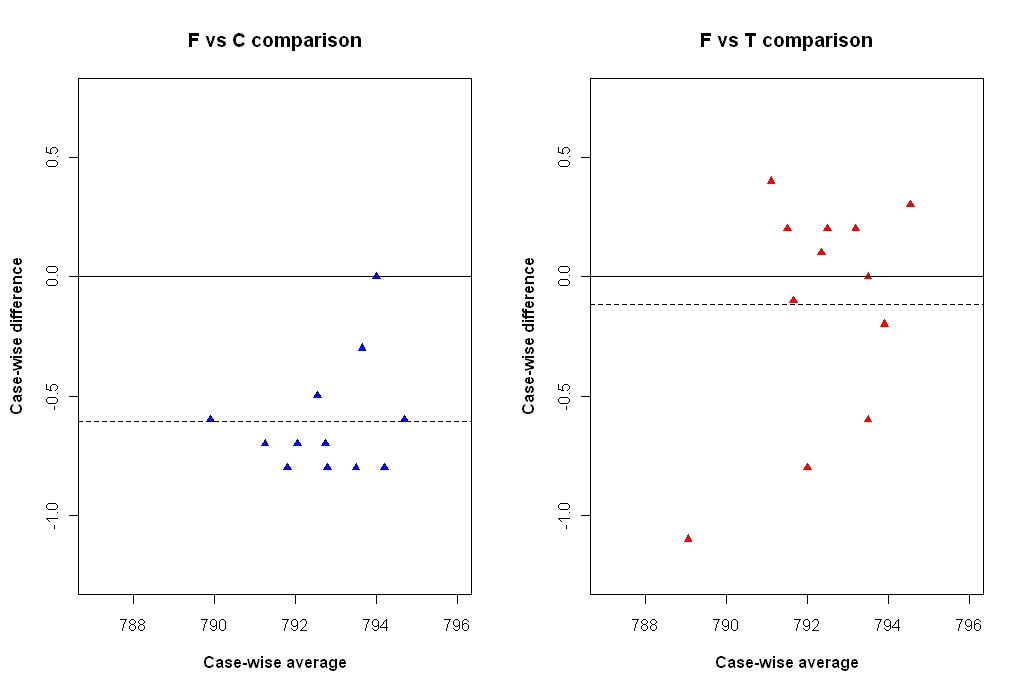
\includegraphics[height=90mm]{GrubbsDataTwoBAplots.jpeg}
  \caption{Bland-Altman plots for Grubbs' F vs C and F vs T comparisons.}\label{GrubbsDataTwoBAplots}
\end{center}
\end{figure}

By inspection, there exists a larger inter-method bias in the `F
vs C' comparison than in the `F vs T' comparison. Conversely there
appears to be less precision in`F vs T' comparison, as indicated
by the greater dispersion of co-variates.

Figures 1.4, 1.5 and 1.6 are three prototype Bland-Altman plots
derived from simulated data, each for the purpose of demonstrating
how the plot would inform an analyst of features that would
adversely affect use of the recommended methodology.

Figure 1.4 demonstrates how the Bland-Altman plot would indicate
increasing variance of differences over the measurement range.
Fitted regression lines, for both the upper and lower half of the
plot, has been added to indicate the trend. Figure 1.5 is an
example of cases where the inter-method bias changes over the
measurement range. This is known as proportional bias. In both
Figures 1.4 and 1.5, the assumptions necessary for further
analysis using the limits of agreement are violated.

Application of regression techniques to the Bland-Altman plot, and
subsequent formal testing for the constant variability of
differences is informative. The data set may be divided into two
subsets, containing the observations wherein the difference values
are less than and greater than the inter-method bias respectively.
For both of these fits, hypothesis tests for the respective slopes
can be performed. While both tests can be considered separately,
multiple comparison procedures, such as the Benjamini-Hochberg
\citep{BH} test, should be also be used.

\begin{figure}[h!]
\begin{center}
  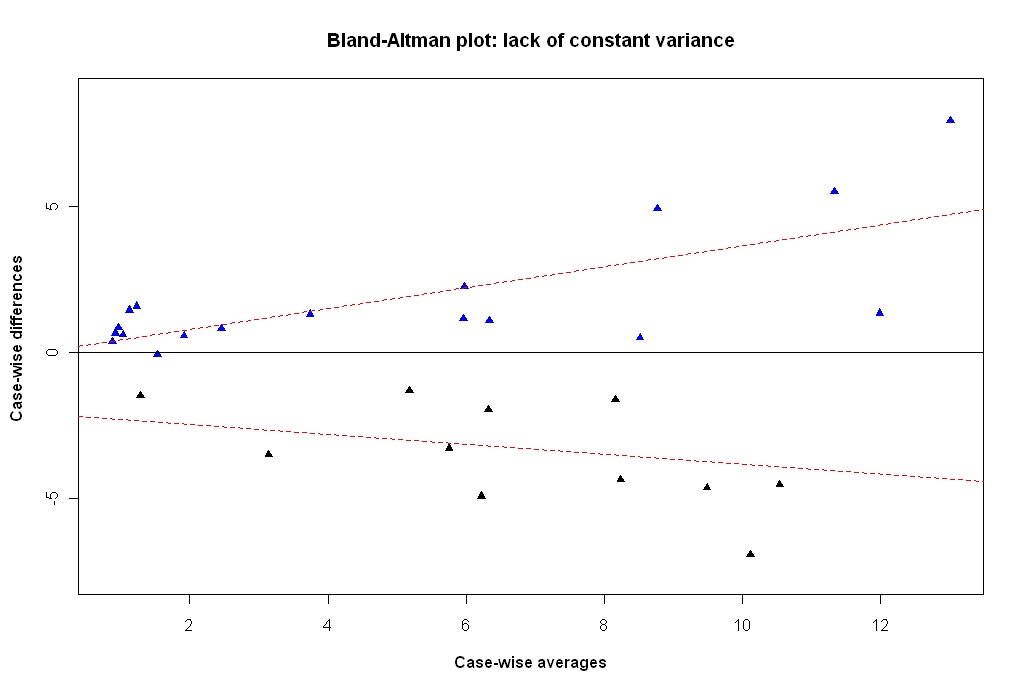
\includegraphics[height=90mm]{BAFanEffect.jpeg}
  \caption{Bland-Altman plot demonstrating the increase of variance over the range.}\label{BAFanEffect}
\end{center}
\end{figure}

\begin{figure}[h!]
\begin{center}
  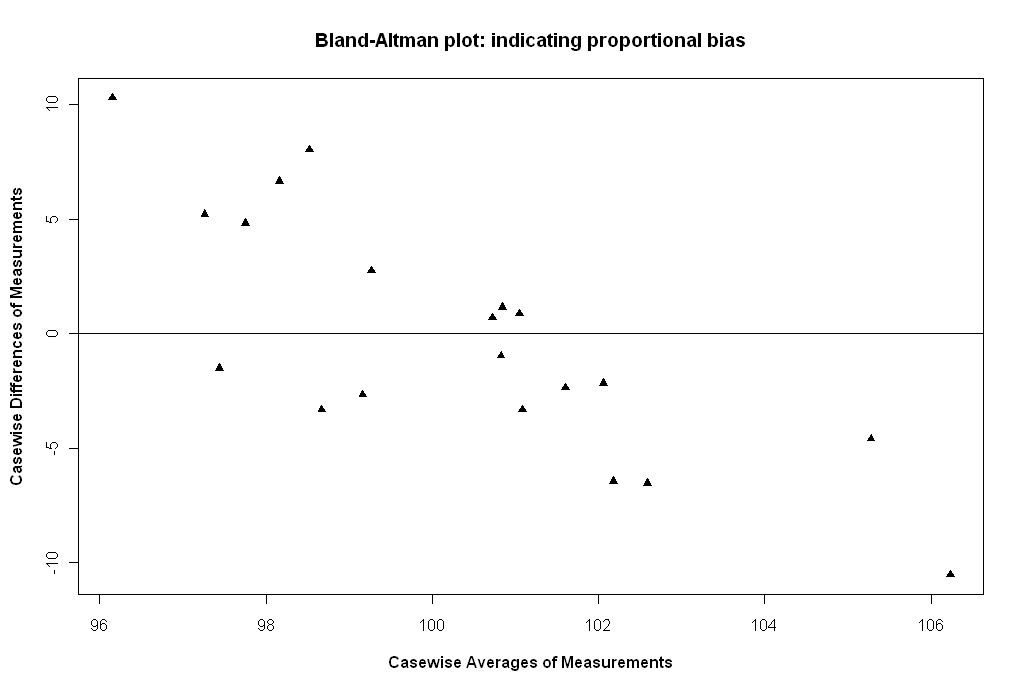
\includegraphics[height=90mm]{PropBias.jpeg}
  \caption{Bland-Altman plot indicating the presence of proportional bias.}\label{PropBias}
\end{center}
\end{figure}

\begin{figure}[h!]
\begin{center}
  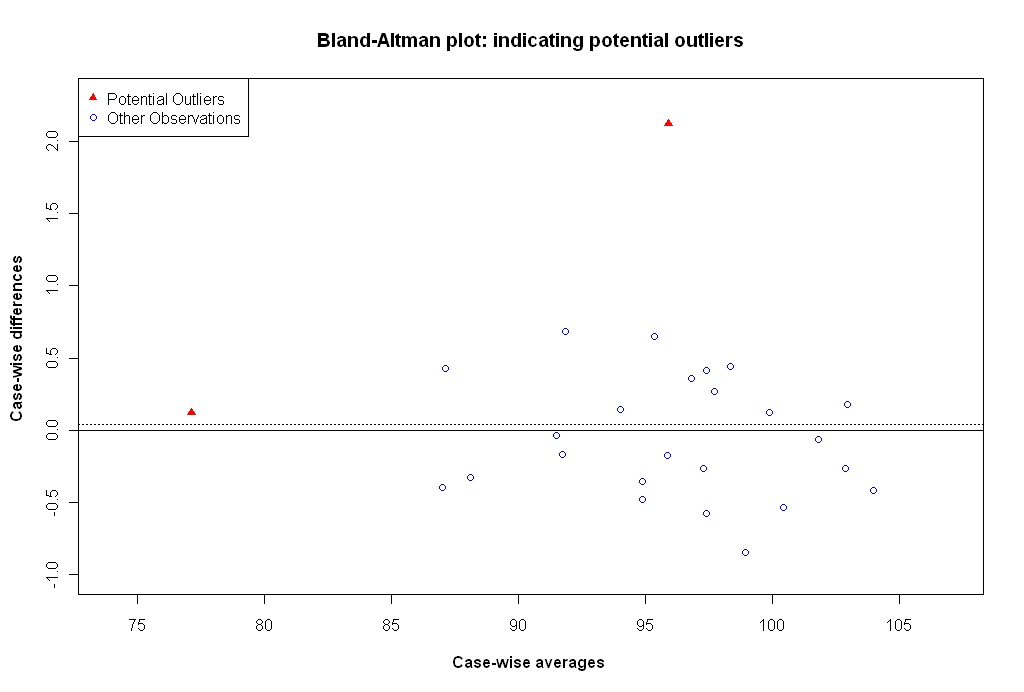
\includegraphics[width=125mm]{BAOutliers.jpeg}
  \caption{Bland-Altman plot indicating the presence of potential outliers.}\label{Outliers}
\end{center}
\end{figure}


% outliers


The Bland-Altman plot also can be used to identify outliers. An
outlier is an observation that is conspicuously different from the
rest of the data that it arouses suspicion that it occurs due to a
mechanism, or conditions, different to that of the rest of the
observations. Classification of outliers can be determined with
numerous established approaches, such as the Grubb's test, but
always classification must be informed by the logic of the data's
formulation. Figure 1.6 is a Bland-Altman plot with two potential
outliers.


\citet*{BA99} do not recommend excluding outliers from analyses,
but remark that recalculation of the inter-method bias estimate,
and further calculations based upon that estimate, are useful for
assessing the influence of outliers. The authors remark that `we
usually find that this method of analysis is not too sensitive to
one or two large outlying differences'.


%\citet{Grubbs} defined an outlier as a co-variate that appears to
%deviate markedly from other members of the sample in which it
%occurs.

In classifying whether a observation from a univariate data set is
an outlier, Grubbs' outlier test is widely used. In assessing
whether a co-variate in a Bland-Altman plot is an outlier, this
test is useful when applied to the difference values treated as a
univariate data set. For Grubbs' data, this outlier test is
carried out on the differences, yielding the following results.

The null and alternative hypotheses is the absence and presence of
at least one outlier respectively. Grubbs' outlier test statistic
$G$ is the largest absolute deviation from the sample mean divided
by the standard deviation of the differences. For the `F vs C'
comparison, $G = 3.6403$. The critical value is calculated using
Student's $t$ distribution and the sample size,
\begin{equation}
U = \frac{n-1}{\sqrt{n}} \sqrt{\frac{t_{\alpha/(2n),n-2}^2}{n - 2
+ t_{\alpha/(2n),n-2}^2}}.
\end{equation}

For this test $U = 0.7501$. The conclusion of this test is that
the fourth observation in the `F vs C' comparison is an outlier,
with $p-value = 0.002799$.

As a complement to the Bland-Altman plot, \citet{Bartko} proposes
the use of a bivariate confidence ellipse, constructed for a
predetermined level.

The minor axis relates to the between subject variability, whereas
the major axis relates to the error mean square, with the ellipse
depicting the size of both relative to each
other.\citet{AltmanEllipse} provides the relevant calculations for
the ellipse. Bartko states that the ellipse can, inter alia, be
used to detect the presence of outliers (furthermore
\citet{Bartko} proposes formal testing procedures, that shall be
discussed in due course). Inspection of Figure 1.7 shows that the
fourth observation is outside the bounds of the ellipse,
concurring with the conclusion that it is an outlier.


\begin{figure}[h!]
  % Requires \usepackage{graphicx}
  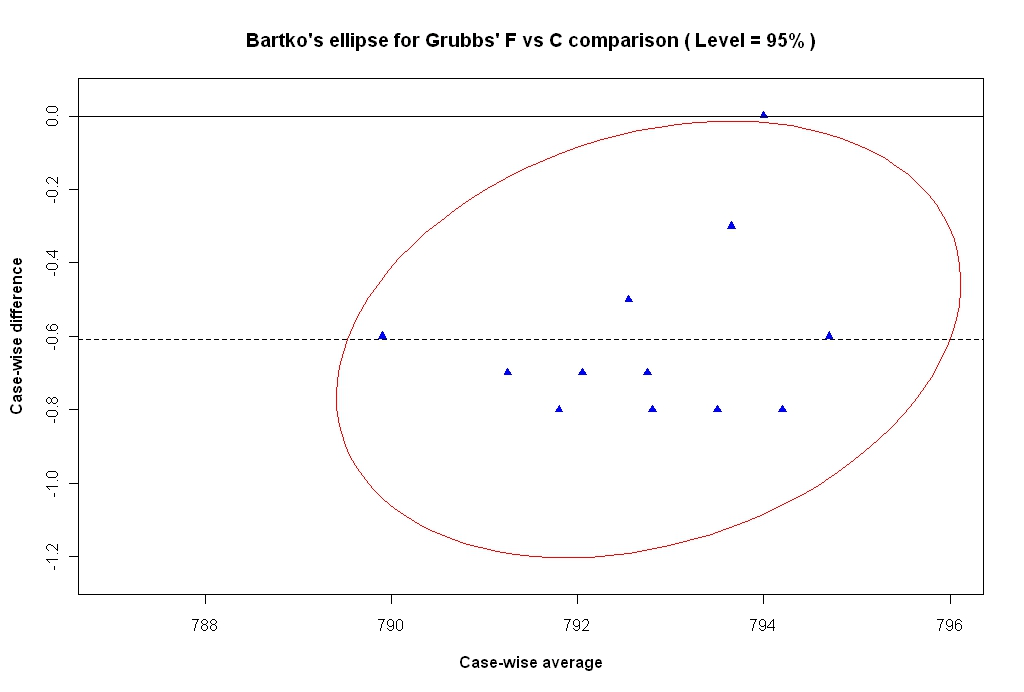
\includegraphics[width=130mm]{GrubbsBartko.jpeg}
  \caption{Bartko's Ellipse For Grubbs' Data.}\label{GrubbsBartko}
\end{figure}

The limitations of using bivariate approaches to outlier detection
in the Bland-Altman plot can demonstrated using Bartko's ellipse.
A co-variate is added to the `F vs C' comparison that has a
difference value equal to the inter-method bias, and an average
value that markedly deviates from the rest of the average values
in the comparison, i.e. 786. Table 1.8 depicts a $95\%$ confidence
ellipse for this enhanced data set. By inspection of the
confidence interval, a conclusion would be reached that this extra
co-variate is an outlier, in spite of the fact that this
observation is consistent with the intended conclusion of the
Bland-Altman plot.

\begin{figure}[h!]
  % Requires \usepackage{graphicx}
  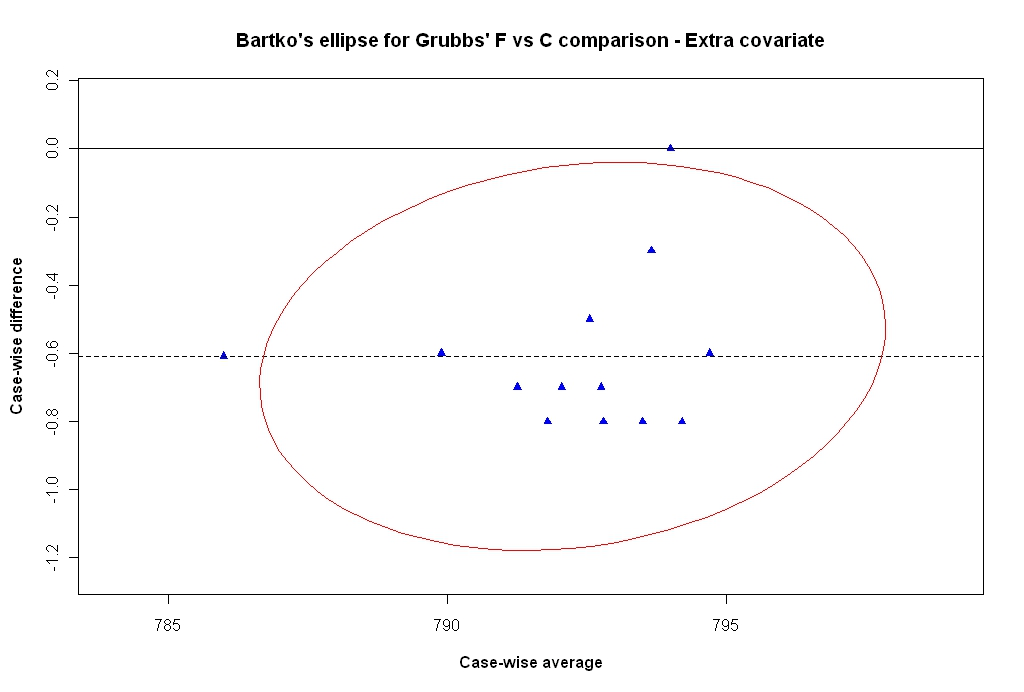
\includegraphics[width=130mm]{GrubbsBartko2.jpeg}
  \caption{Bartko's Ellipse For Grubbs' Data, with an extra covariate.}\label{GrubbsBartko2}
\end{figure}

In the Bland-Altman plot, the horizontal displacement of any
observation is supported by two independent measurements. Any
observation should not be considered an outlier on the basis of a
noticeable horizontal displacement from the main cluster, as in
the case with the extra co-variate. Conversely, the fourth
observation, from the original data set, should be considered an
outlier, as it has a noticeable vertical displacement from the
rest of the observations.

Bartko's ellipse provides a visual aid to determining the
relationship between variances. If $\mbox{var}(a_{i})$ is greater
than $\mbox{var}(d_{i})$, the orientation of the ellipse is
horizontal. Conversely if $\mbox{var}(a_{i})$ is less than
$\mbox{var}(d_{i})$, the orientation of the ellipse is vertical.
\newpage



%\begin{figure}[h!]
%\begin{center}
%  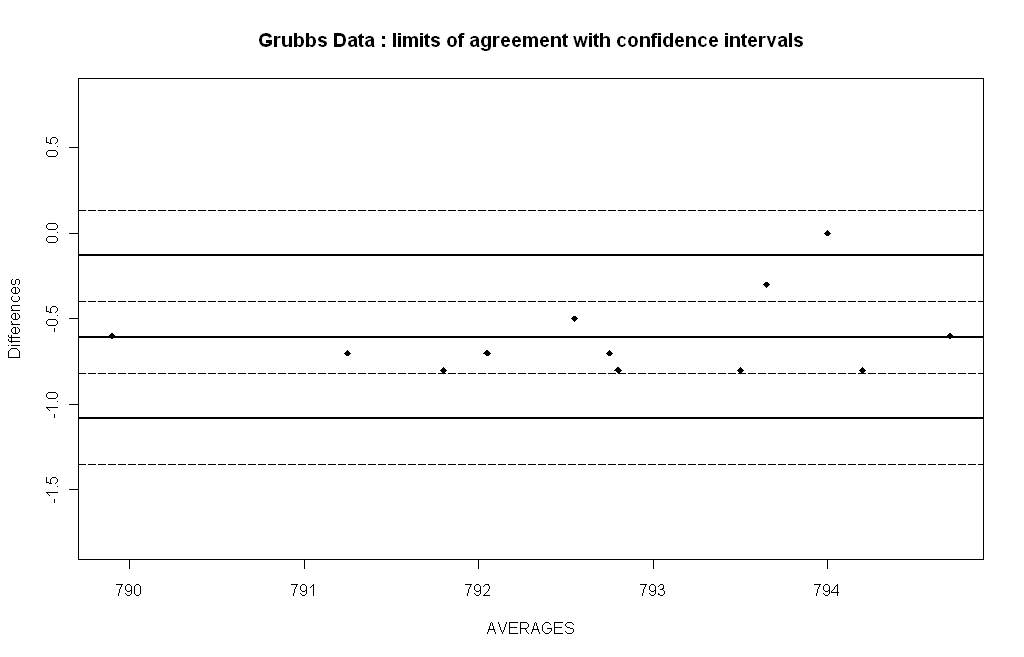
\includegraphics[width=125mm]{GrubbsLOAwCIs.jpeg}
%  \caption{Limits of agreement with confidence intervals}\label{LOAwCIs}
%\end{center}
%\end{figure}

\subsection{Variations of the Bland-Altman Plot} Referring to the
assumption that bias and variability are constant across the range
of measurements, \citet{BA99} address the case where there is an
increase in variability as the magnitude increases. They remark
that it is possible to ignore the issue altogether, but the limits
of agreement would wider apart than necessary when just lower
magnitude measurements are considered. Conversely the limits would
be too narrow should only higher magnitude measurements be used.
To address the issue, they propose the logarithmic transformation
of the data. The plot is then formulated as the difference of
paired log values against their mean. Bland and Altman acknowledge
that this is not easy to interpret, and may not be suitable in
all cases.

\citet{BA99} offers two variations of the Bland-Altman plot that
are intended to overcome potential problems that the conventional
plot would inappropriate for. The first variation is a plot of
casewise differences as percentage of averages, and is appropriate
when there is an increase in variability of the differences as the
magnitude increases. The second variation is a plot of casewise
ratios as percentage of averages. This will remove the need for
log transformation. This approach is useful when there is an
increase in variability of the differences as the magnitude of the
measurement increases. \citet{Eksborg} proposed such a ratio plot,
independently of Bland and Altman. \citet{Dewitte} commented on
the reception of this article by saying `Strange to say,this
report has been overlooked'.




\subsection{Regression-based Limits of Agreement} Assuming that
there will be no curvature in the scatter-plot, the methodology
regresses the difference of methods ($d$) on the average of those
methods ($a$) with a simple intercept slope model; $\hat{d} =
b_{0}+ b_{1}a.$ Should the slope $b_{1}$ be found to be
negligible, $\hat{d}$ takes the value $\bar{d}$.

The next step to take in calculating the limits is also a
regression, this time of the residuals as a function of the scale
of the measurements, expressed by the averages $a_{i}$;
 $ \hat{R} = c_{0}+ c_{1}a_{i}$

With reference to absolute values following a half-normal
distribution with mean $\sigma\sqrt{\frac{2}{\pi}}$, \citet{BA99} formulate the regression based limits of agreement as
follows
 \begin{equation}
  \hat{d} \pm 1.96\sqrt{\frac{\pi}{2}}\hat{R} = \hat{d} \pm 2.46\hat{R}
 \end{equation}

\subsection{Replicate Measurements}

Thus far, the formulation for comparison of two measurement
methods is one where one measurement by each method is taken on
each subject. Should there be two or more measurements by each
methods, these measurement are known as `replicate measurements'.
\citet{BXC2008} recommends the use of replicate measurements, but
acknowledges that  additional computational complexity.

\citet*{BA86} address this problem by offering two different
approaches. The premise of the first approach is that replicate
measurements can be treated as independent measurements. The
second approach is based upon using the mean of the each group of
replicates as a representative value of that group. Using either
of these approaches will allow an analyst to estimate the inter
method bias.

%\subsubsection{Mean of Replicates Limits of Agreement}

However, because of the removal of the effects of the replicate
measurements error, this would cause the estimation of the
standard deviation of the differences to be unduly small.
\citet*{BA86} propose a correction for this.

\citet{BXC2008} takes issue with the limits of agreement based on
mean values, in that they can only be interpreted as prediction
limits for difference between means of repeated measurements by
both methods, as opposed to the difference of all measurements.
Incorrect conclusions would be caused by such a misinterpretation.
\citet{BXC2008} demonstrates how the limits of agreement
calculated using the mean of replicates are `much too narrow as
prediction limits for differences between future single
measurements'. This paper also comments that, while treating the
replicate measurements as independent will cause a downward bias
on the limits of agreement calculation, this method is preferable
to the `mean of replicates' approach.

The approach proposed by \citet{BA83} is a formal test on the
Pearson correlation coefficient of case-wise differences and means
($\rho_{ad}$). According to the authors, this test is equivalent
to the `Pitman Morgan Test'. For the Grubbs data, the correlation
coefficient estimate ($r_{ad}$) is 0.2625, with a 95\% confidence
interval of (-0.366, 0.726) estimated by Fishers `r to z'
transformation \citep*{Cohen}. The null hypothesis ($\rho_{ad}$
=0)would fail to be rejected. Consequently the null hypothesis of
equal variances of each method would also fail to be rejected.
There has no been no further mention of this particular test in
\citet{BA86}, although \citet{BA99} refers to Spearman's rank
correlation coefficient. \citet{BA99} comments `we do not see a
place for methods of analysis based on hypothesis testing'.
\citet{BA99} also states that consider structural equation models
to be inappropriate.

\citet{DunnSEME} highlights an important issue regarding using
models such as these, the identifiability problem. This comes as a
result of there being too many parameters to be estimated.
Therefore assumptions about some parameters, or estimators used,
must be made so that others can be estimated. For example $\alpha$
may take the value of the inter-method bias estimate from
Bland-Altman methodology. Another assumption is that the precision
ratio $\lambda=\frac{\sigma^{2}_{\epsilon}}{\sigma^{2}_{\delta}}$
may be known.


\citet{DunnSEME} considers methodologies based on two methods with single measurements on each subject as inadequate for a serious study
on the measurement characteristics of the methods. This is because there would not be enough data to allow for a meaningful analysis.
There is, however, a contrary argument that is very difficult to get replicate
observations when the measurement method requires invasive medical procedure.

\citet{DunnSEME} recommends the following approach for analyzing
method comparison data. Firstly he recommends conventional
Bland-Altman methodology; plotting the scatterplot and the
Bland-Altman plot, complemented by estimate for the limits of
agreement and the correlation coefficient between the difference
and the mean. Additionally boxplots may be useful in considering
the marginal distributions of the observations. The second step is
the calculations of summary statistics; the means and variances of
each set of measurements, and the covariances.
%Should covariance values be greater than the either of the two variances,

When both methods measure in the same scale (i.e. $\beta = 1$),
\citet{DunnSEME} recommends the use of Grubbs estimators to
estimate error variances, and to test for their equality. A test
of whether the intercept $\alpha$ may be also be appropriate.



%This application of the
%Grubbs method presumes the existence of this condition, and necessitates
%replication of observations by means external to and independent of the first
%means. The Grubbs estimators method is based on the laws of propagation of
%error. By making three independent simultaneous measurements on the same
%physical material, it is possible by appropriate mathematical manipulation of
%the sums and differences of the associated variances to obtain a valid
%estimate of the precision of the primary means. Application of the Grubbs
%estimators procedure to estimation of the precision of an apparatus uses
%the results of a physical test conducted in such a way as to obtain a series
%of sets of three independent observations.



%%%%%%%%%%%%%%%%%%%%%%%%%%%%%%%%%%%%%%%%%%%%%%%%%%%%%%%%%%%%%%%%%%%%%%%%%%%%%%%%%%%%%%%%%%%%%%%%%%%%%%%%

%%%%%%%%%%%%%%%%%%%%%%%%%%%%%%%%%%%%%%%%%%%%%%%%%%%%%%%%%%%%%%%%%%%%%%%%%%%%%%%%%%%%%%%%%%%%%%%%%%%%%%%%
\newpage

%%%%%%%%%%%%%%%%%%%%%%%%%%%%%%%%%%%%%%%%%%%%%%%%%%%%%%%%%%%%%%%%%%%%%%%%%%%%%%%%%%%%%%%%%%%%%%%%%%%%%%%%%%%%%%%%%%


\chapter{Linear Mixed Effects Models}

\section{LME models in Method comparison}
%With the greater computing power available for scientific
%analysis, it is inevitable that complex models such as linear
%mixed effects models should be applied to method comparison
%studies.







% \begin{equation}
% data here
% \end{equation}

\newpage
\section{Lai Shiao}
\citet{LaiShiao} use mixed models to determine the factors that
affect the difference of two methods of measurement using the
conventional formulation of linear mixed effects models.

If the parameter \textbf{b}, and the variance components are not
significantly different from zero, the conclusion that there is no
inter-method bias can be drawn. If the fixed effects component
contains only the intercept, and a simple correlation coefficient
is used, then the estimate of the intercept in the model is the
inter-method bias. Conversely the estimates for the fixed effects
factors can advise the respective influences each factor has on
the differences. The Proc Mixed package allows users to specify
different correlation structures of the variance components
\textbf{G} and \textbf{R}.


Oxygen saturation is one of the most frequently measured variables
in clinical nursing studies. `Fractional saturation' ($HbO_{2}$)
is considered to be the gold standard method of measurement, with
`functional saturation' ($SO_{2}$) being an alternative method.
The method of examining the causes of differences between these
two methods is applied to a clinical study conducted by
\citet{Shiao}. This experiment was conducted by 8 lab
practitioners on blood samples, with varying levels of
haemoglobin, from two donors. The samples have been in storage for
varying periods ( described by the variable `Bloodage') and are
categorized according to haemoglobin percentages(i.e
$0\%$,$20\%$,$40\%$,$60\%$,$80\%$,$100\%$). There are 625
observations in all.

\citet{LaiShiao} fits two models on this data, with the lab
technicians and the replicate measurements as the random effects
in both models. The first model uses haemoglobin level as a fixed
effects component. For the second model, blood age is added as a
second fixed factor.

\subsubsection{Single fixed effect} The first model fitted by \citet{LaiShiao} takes the
blood level as the sole fixed effect to be analyzed. The following
coefficient estimates are estimated by `Proc Mixed';
\begin{eqnarray}
\mbox{fixed effects :   } 2.5056 - 0.0263\mbox{Fhbperct}_{ijtl} \\
(\mbox{p-values :   } = 0.0054, <0.0001, <0.0001)\nonumber\\\nonumber\\
\mbox{random effects :   } u(\sigma^{2}=3.1826) + e_{ijtl}
(\sigma^{2}_{e}=0.1525, \rho= 0.6978) \nonumber\\
(\mbox{p-values :   } = 0.8113, <0.0001, <0.0001)\nonumber
\end{eqnarray}

With the intercept estimate being both non-zero and statistically
significant ($p=0.0054$), this models supports the presence
inter-method bias is $2.5\%$ in favour of $SO_{2}$. Also, the
negative value of the haemoglobin level coefficient indicate that
differences will decrease by $0.0263\%$ for every percentage
increase in the haemoglobin .

In the random effects estimates, the variance due to the
practitioners is $3.1826$, indicating that there is a significant
variation due to technicians ($p=0.0311$) affecting the
differences. The variance for the estimates is given as $0.1525$,
($p<0.0001$).

\subsubsection{Two fixed effects}
Blood age is added as a second fixed factor to the model,
whereupon new estimates are calculated;
\begin{eqnarray}
\mbox{fixed effects :   } -0.2866 + 0.1072 \mbox{Bloodage}_{ijtl}
- 0.0264\mbox{Fhbperct}_{ijtl}\nonumber\\
( \mbox{p-values :   } = 0.8113, <0.0001, <0.0001)\nonumber\\\nonumber\\
\mbox{random effects :   } u(\sigma^{2}=10.2346) + e_{ijtl}
(\sigma^{2}_{e}=0.0920, \rho= 0.5577) \nonumber\\
(\mbox{p-values :   } = 0.0446, <0.0001, <0.0001)
\end{eqnarray}


With this extra fixed effect added to the model, the intercept
term is no longer statistically significant. Therefore, with the
presence of the second fixed factor, the model is no longer
supporting the presence of inter-method bias. Furthermore, the
second coefficient indicates that the blood age of the observation
has a significant bearing on the size of the difference between
both methods ($p <0.0001$). Longer storage times for blood will
lead to higher levels of particular blood factors such as MetHb
and HbCO (due to the breakdown and oxidisation of the
haemoglobin). Increased levels of MetHb and HbCO are concluded to
be the cause of the differences. The coefficient for the
haemoglobin level doesn't differ greatly from the single fixed
factor model, and has a much smaller effect on the differences.
The random effects estimates also indicate significant variation
for the various technicians; $10.2346$ with $p=0.0446$.

\citet{LaiShiao} demonstrates how that linear mixed effects models
can be used to provide greater insight into the cause of the
differences. Naturally the addition of further factors to the
model provides for more insight into the behavior of the data.











\addcontentsline{toc}{section}{Bibliography}

\bibliography{transferbib}
\end{document}
